\documentclass[journal,twoside,web]{ieeecolor}
\usepackage{tmi}
\usepackage{amsmath,amssymb,amsfonts}
\usepackage{algorithmic}
\usepackage{graphicx}
\graphicspath{{images}}
\usepackage{textcomp}
\def\BibTeX{{\rm B\kern-.05em{\sc i\kern-.025em b}\kern-.08em
    T\kern-.1667em\lower.7ex\hbox{E}\kern-.125emX}}
\markboth{\journalname, VOL. XX, NO. XX, XXXX 2020}
{Author \MakeLowercase{\textit{et al.}}: Preparation of Papers for IEEE TRANSACTIONS ON MEDICAL IMAGING}

\begin{document}
\title{Verarbeitung von Gesichtsaufnahmen zur Genderklassifikation als Anwendung neuronaler Netze}
\author{Niklas Herhoffer, Celine Schneider, Andreas Braig
\thanks{Diese Arbeit wurde im Rahmen des Kurses TEL22AT1 erstellt.}
\thanks{Diese Arbeit wurde am 02.03.2025 eingereicht.}  
\thanks{Die Autoren sind Studierende an der Dualen Hochschule Baden-Württemberg Mannheim.}}

\maketitle

\begin{abstract}
    Diese Arbeit untersucht die Anwendung neuronaler Netze zur Genderklassifikation von Gesichtsaufnahmen. Hierbei wird ein Convolutional Neural Network (CNN) verwendet, um das Geschlecht abgebildeter Personen basierend auf vorab segmentierten und verarbeiteten Gesichtsaufnahmen zu klassifizieren. Das Ziel dieser Arbeit ist es, den Prozess der Bildverarbeitung und Klassifikation effizient zu gestalten.
\end{abstract}


\begin{IEEEkeywords}
    Neuronales Netz, Bildsegmentierung, Convolutional Neural Network, Genderklassifikation, Deep Learning
\end{IEEEkeywords}

\section{Einleitung}
\label{sec:introduction}
\IEEEPARstart{D}{iese} Arbeit befasst sich mit der Verarbeitung und Klassifikation von Gesichtsaufnahmen. Die verwendeten Daten bestehen aus Gesichtsaufnahmen von Personen unterschiedlichen Alters. 

Die erste Teilaufgabe der Arbeit besteht in der Segmentierung und Verarbeitung des Datensatzes, um die Gesichtselemente (insbesondere Augen und Mund) in den Bildern einheitlich zu positionieren. Dies wird erreicht, indem ein gleichschenkliges Dreieck mit festen Positionen für die Augen und den Mund im Bild definiert wird. 

Die zweite Teilaufgabe konzentriert sich auf die Klassifikation des Geschlechts der abgebildeten Person. Ein Convolutional Neural Network wird trainiert, um eine binäre Klassifikation zwischen Männlich (0) und Weiblich (1) durchzuführen.

Für die Implementierung wurde die Programmiersprache Python verwendet, unterstützt durch die Bibliotheken OpenCV, numpy und Pytorch.

\section{Stand der Technik}
In diesem Kapitel wird der aktuelle Stand der Technik zur Bildsegmentierung und Klassifizierung im Kontext von neuronalen Netzen und Bildverarbeitung diskutiert.

\subsection{Bildsegmentierung}
Die Bildsegmentierung ist ein wichtiger Schritt in der Bildverarbeitung, um relevante Merkmale aus den Bildern zu extrahieren. Verschiedene Techniken und Algorithmen werden verwendet, um die Gesichtsmerkmale zu extrahieren und zu standardisieren.

\subsection{Neuronale Netze und Pytorch}
Pytorch hat sich als eine der führenden Deep-Learning-Bibliotheken etabliert. Hier wird die Funktionsweise von Convolutional Neural Networks (CNNs) erklärt, die besonders in der Bildklassifikation erfolgreich eingesetzt werden.

\subsection{Potenziale der Anwendung von Deep Learning}

\section{Datensatz}
In diesem Kapitel wird der verwendete Datensatz detailliert beschrieben. Dabei werden sowohl die Quelle des Datensatzes als auch die Herausforderungen bei der Arbeit mit diesen Daten erläutert.

\subsection{Allgemeine Beschreibung des Datensatzes}
Der Datensatz besteht aus Gesichtsaufnahmen, die von Personen unterschiedlichen Alters und mit unterschiedlichen Gesichtszügen aufgenommen wurden.

\subsection{Herausforderungen bei der Datenverarbeitung}
Bei der Arbeit mit Gesichtsaufnahmen treten Herausforderungen wie die Variation der Beleuchtung, der Gesichtsausdruck und die Position der Kamera auf. Diese müssen vor der Klassifikation in einem Preprocessing-Schritt berücksichtigt werden.

\section{Implementierte Lösung}
In diesem Kapitel wird die entwickelte Lösung zur Segmentierung und Klassifikation beschrieben. Dabei werden die einzelnen Schritte des Prozesses erklärt.

\begin{figure}[!t]
    \centerline{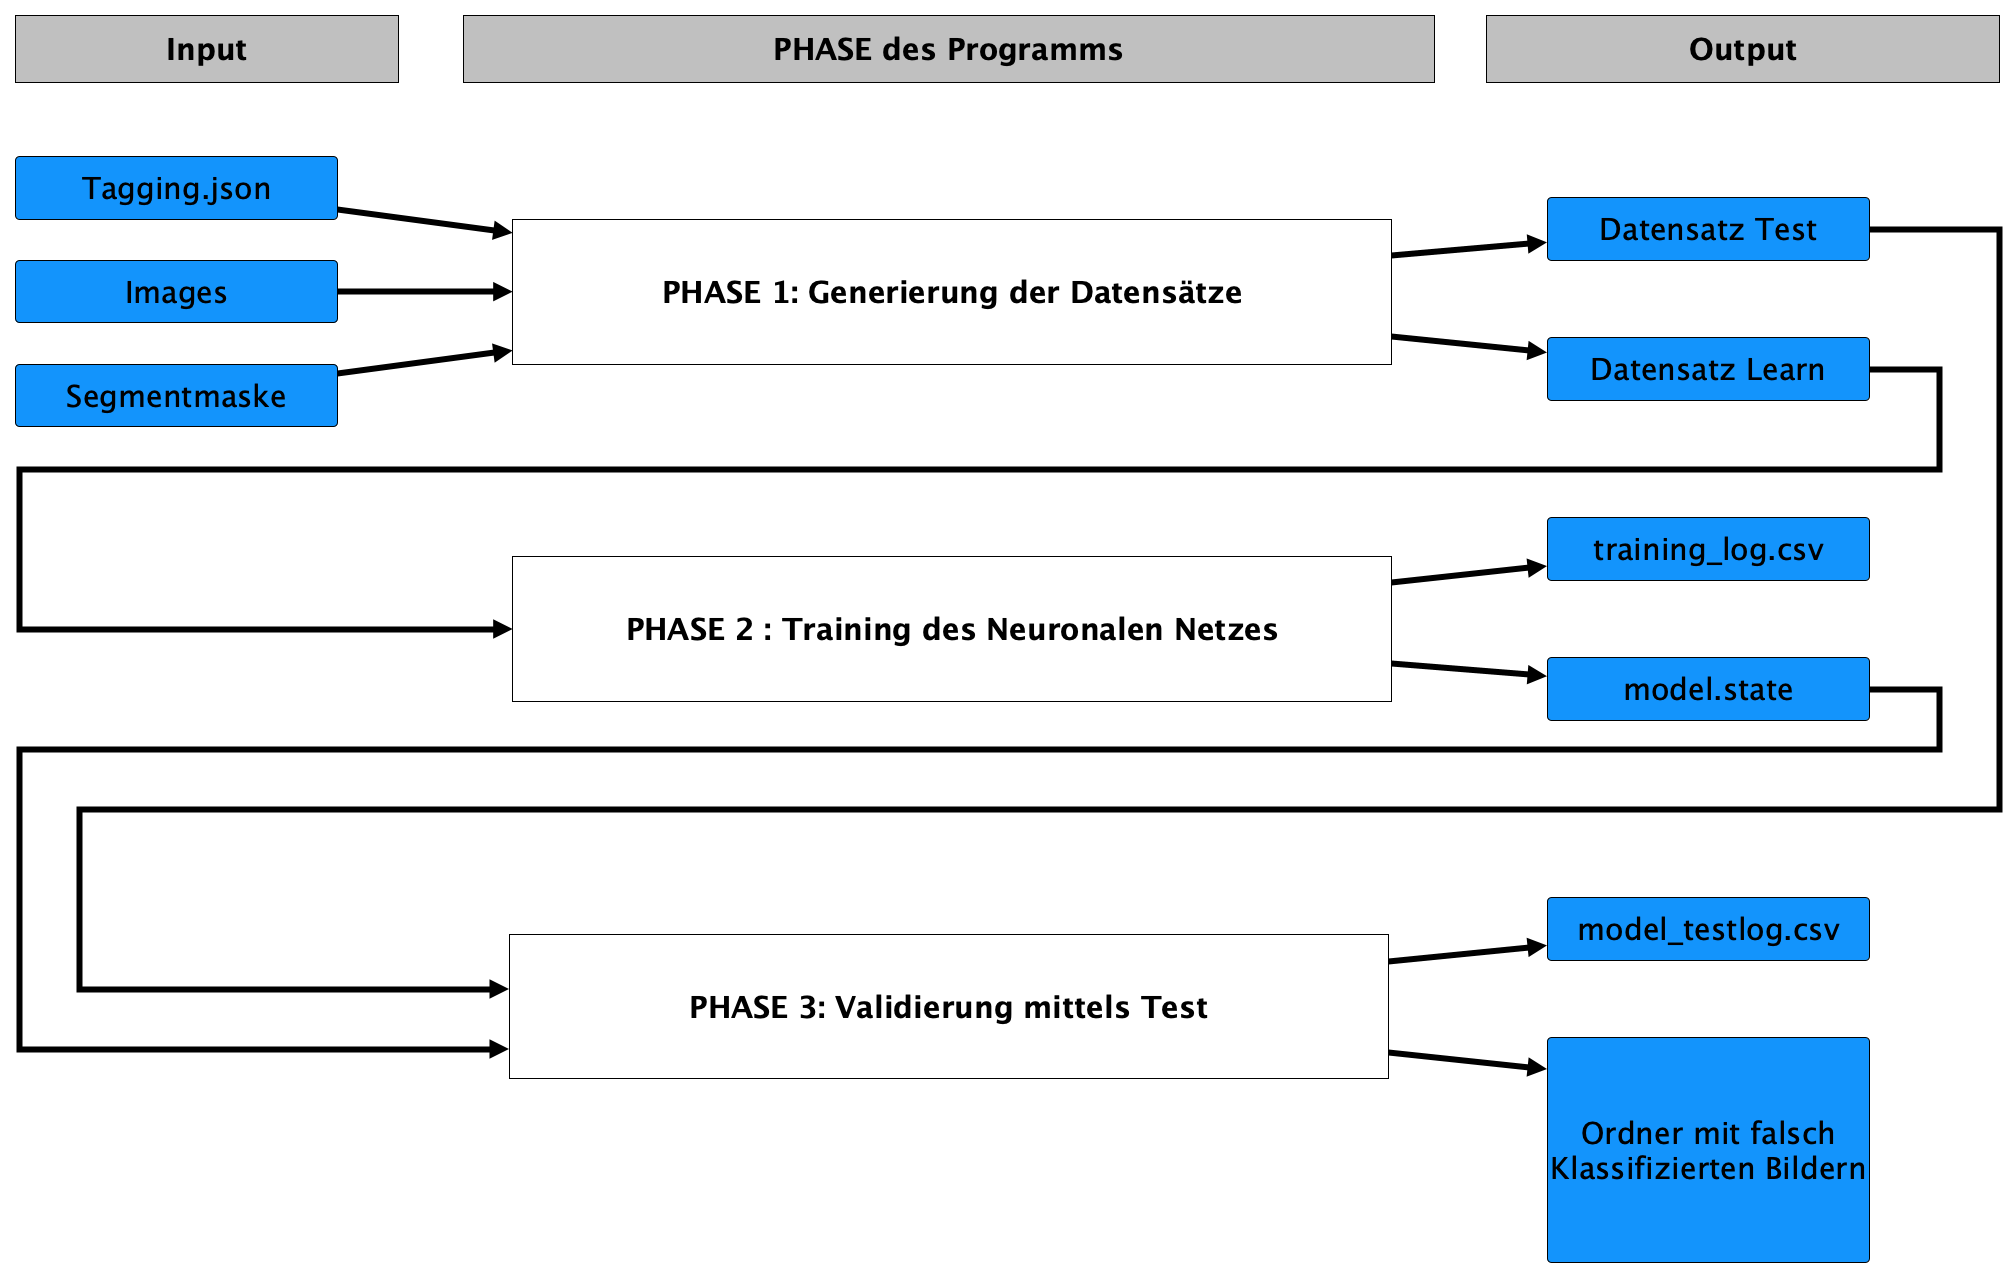
\includegraphics[width=\columnwidth]{Architektur.png}}
    \caption{Darstellung der Programmarchitektur in Form eines Blockschaltbildes}
    \label{fig:architecture}
\end{figure}

\subsection{Preprocessing}
Das Preprocessing übernimmt die zentrale Aufgabe der Vorverarbeitung der Rohdaten für das Training des neuronalen Netzwerks.
Durch die Funktion \texttt{cleanup} wird zunächst sichergestellt, dass sämtliche Datensätze in den Zielordnern gelöscht werden, um eine Vermischung mit einem veralteten Datensatz zu verhindern.
Anschließend werden die Metadaten, einschließlich der Dateinamen und der Geschlechter, aus der \texttt{tag.json} extrahiert und in einem strukturierten 2D-Array gespeichert, sodass die Weiterverarbeitung der Daten erleichtert wird.
Auf Grundlage der so gewonnenen Zuordnungen zwischen Bilddateien und Geschlecht erfolgt die Trennung der Bilddaten in zwei separate Ordner - einen für männliche und einen für weibliche Gesichter.
Im nächsten Schritt wird die Funktion \texttt{freistellen} eingesetzt, um die Gesichter in den Bildern zu extrahieren.
Nach dieser Extraktion erfolgt eine Transformation, die die Gesichter auf eine standardisierte Positionierung von Augen und Mund ausrichtet, um eine konsistente Eingabe für das Modell zu gewährleisten.
Anschließend erfolgt mithilfe der Funktion \texttt{train\_test\_split} die Aufteilung der vorverarbeiteten Bilddaten in Trainings- und Testdatensätze.
Hierbei wird ein zufällig ausge6wählter Prozentsatz der Bilder in den Testdatensatz überführt.
Dieser Schritt ist entscheidend, um eine objektive Evaluierung des Modells zu ermöglichen und Überanpassung (Overfitting) zu vermeiden, wie in Abschnitt \ref{sec:overfitting} beschrieben.

\subsection{Segmentierung}
Im Segmentierungsschritt werden die Gesichtselemente wie Augen, Nase und Mund positioniert und normiert, um das Modell mit konsistenten Eingabedaten zu füttern.

\subsection{CNN Modell}
Das Convolutional Neural Network (CNN) wird verwendet, um das Geschlecht der abgebildeten Person zu klassifizieren. Hierbei kommen mehrere Convolutional Layers und Pooling Layers zum Einsatz, um aus den Eingabebildern tiefere Merkmale zu extrahieren.

\section{Lösungsansätze im Vergleich}
In diesem Abschnitt werden verschiedene Lösungsansätze und Modelle verglichen, die zur Geschlechtsklassifikation verwendet werden können.
\begin{figure}[!t]
    \centerline{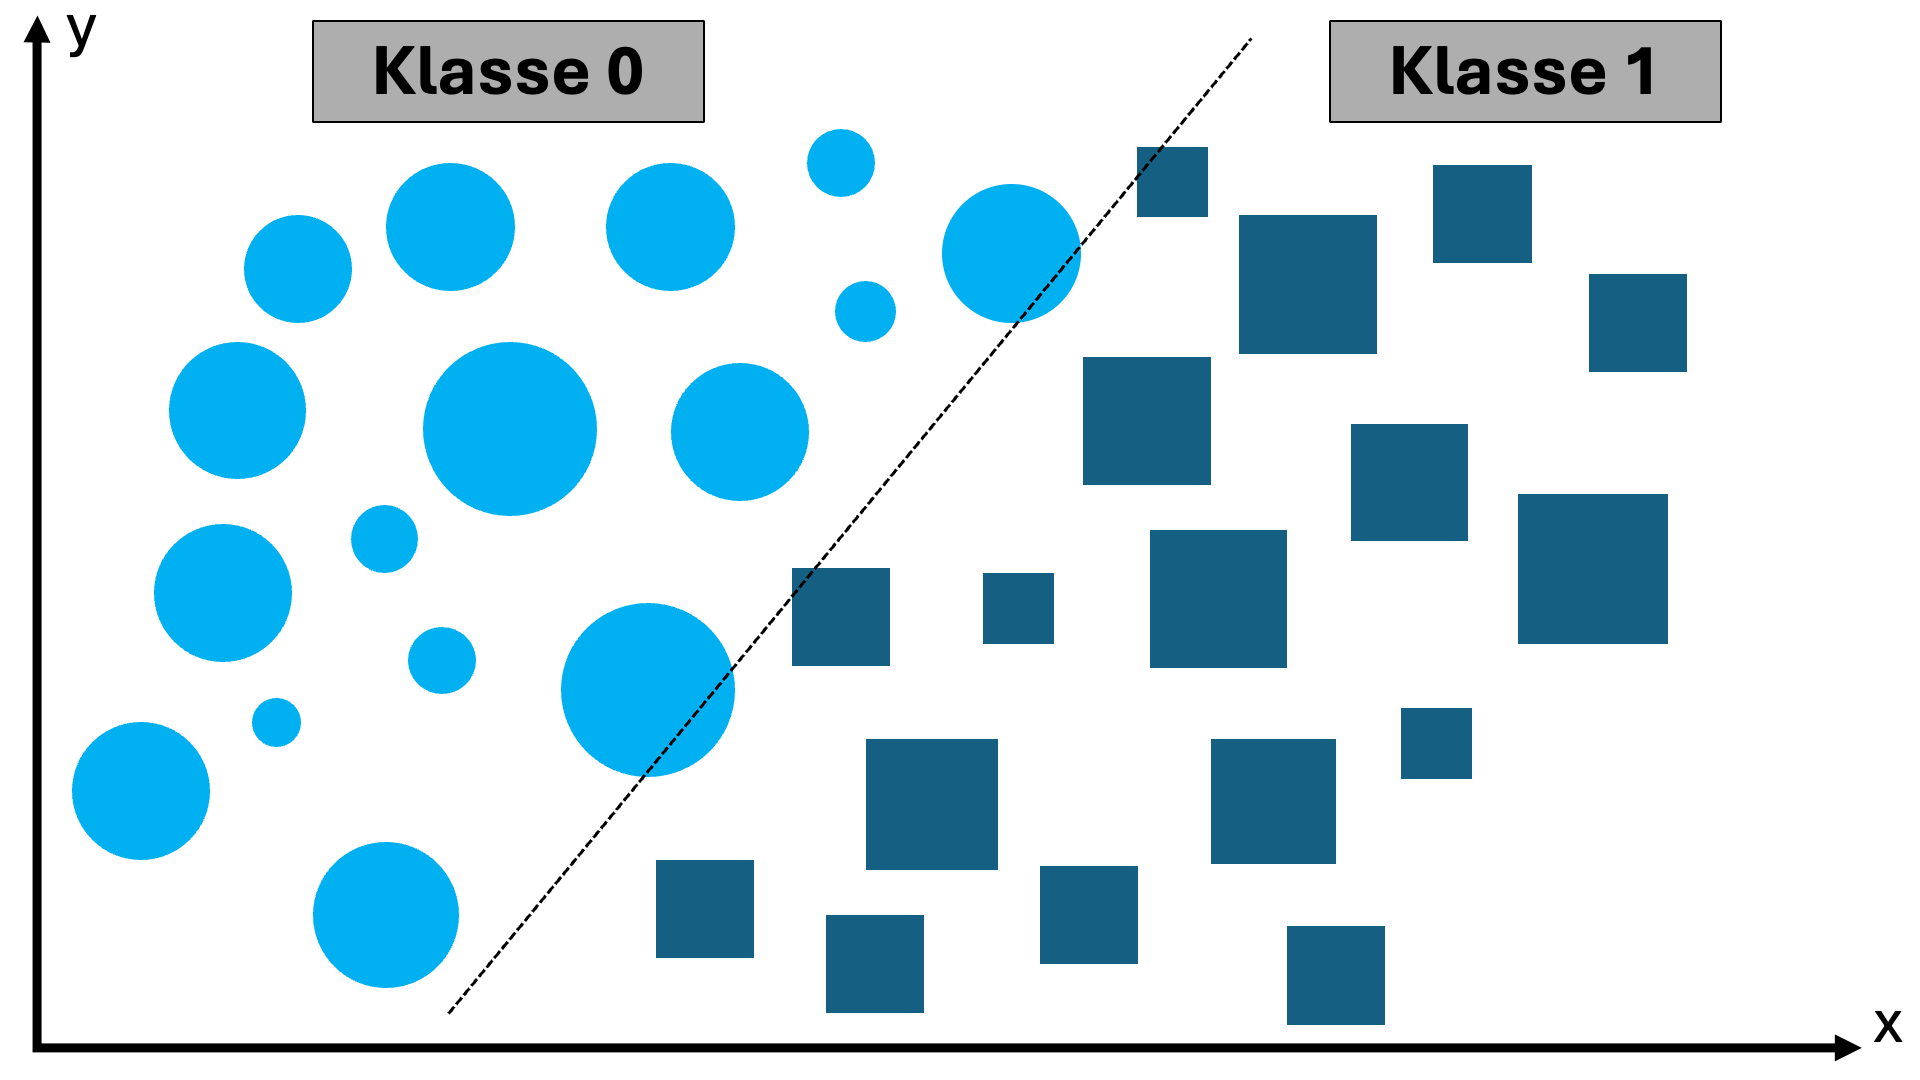
\includegraphics[width=\columnwidth]{Andi/binaere_klassifikation.png}}
    \caption{Beispiel für die binäre Klassifikation.}
    \label{fig:binaere_klassifikation}
\end{figure}

\begin{figure}[!t]
    \centerline{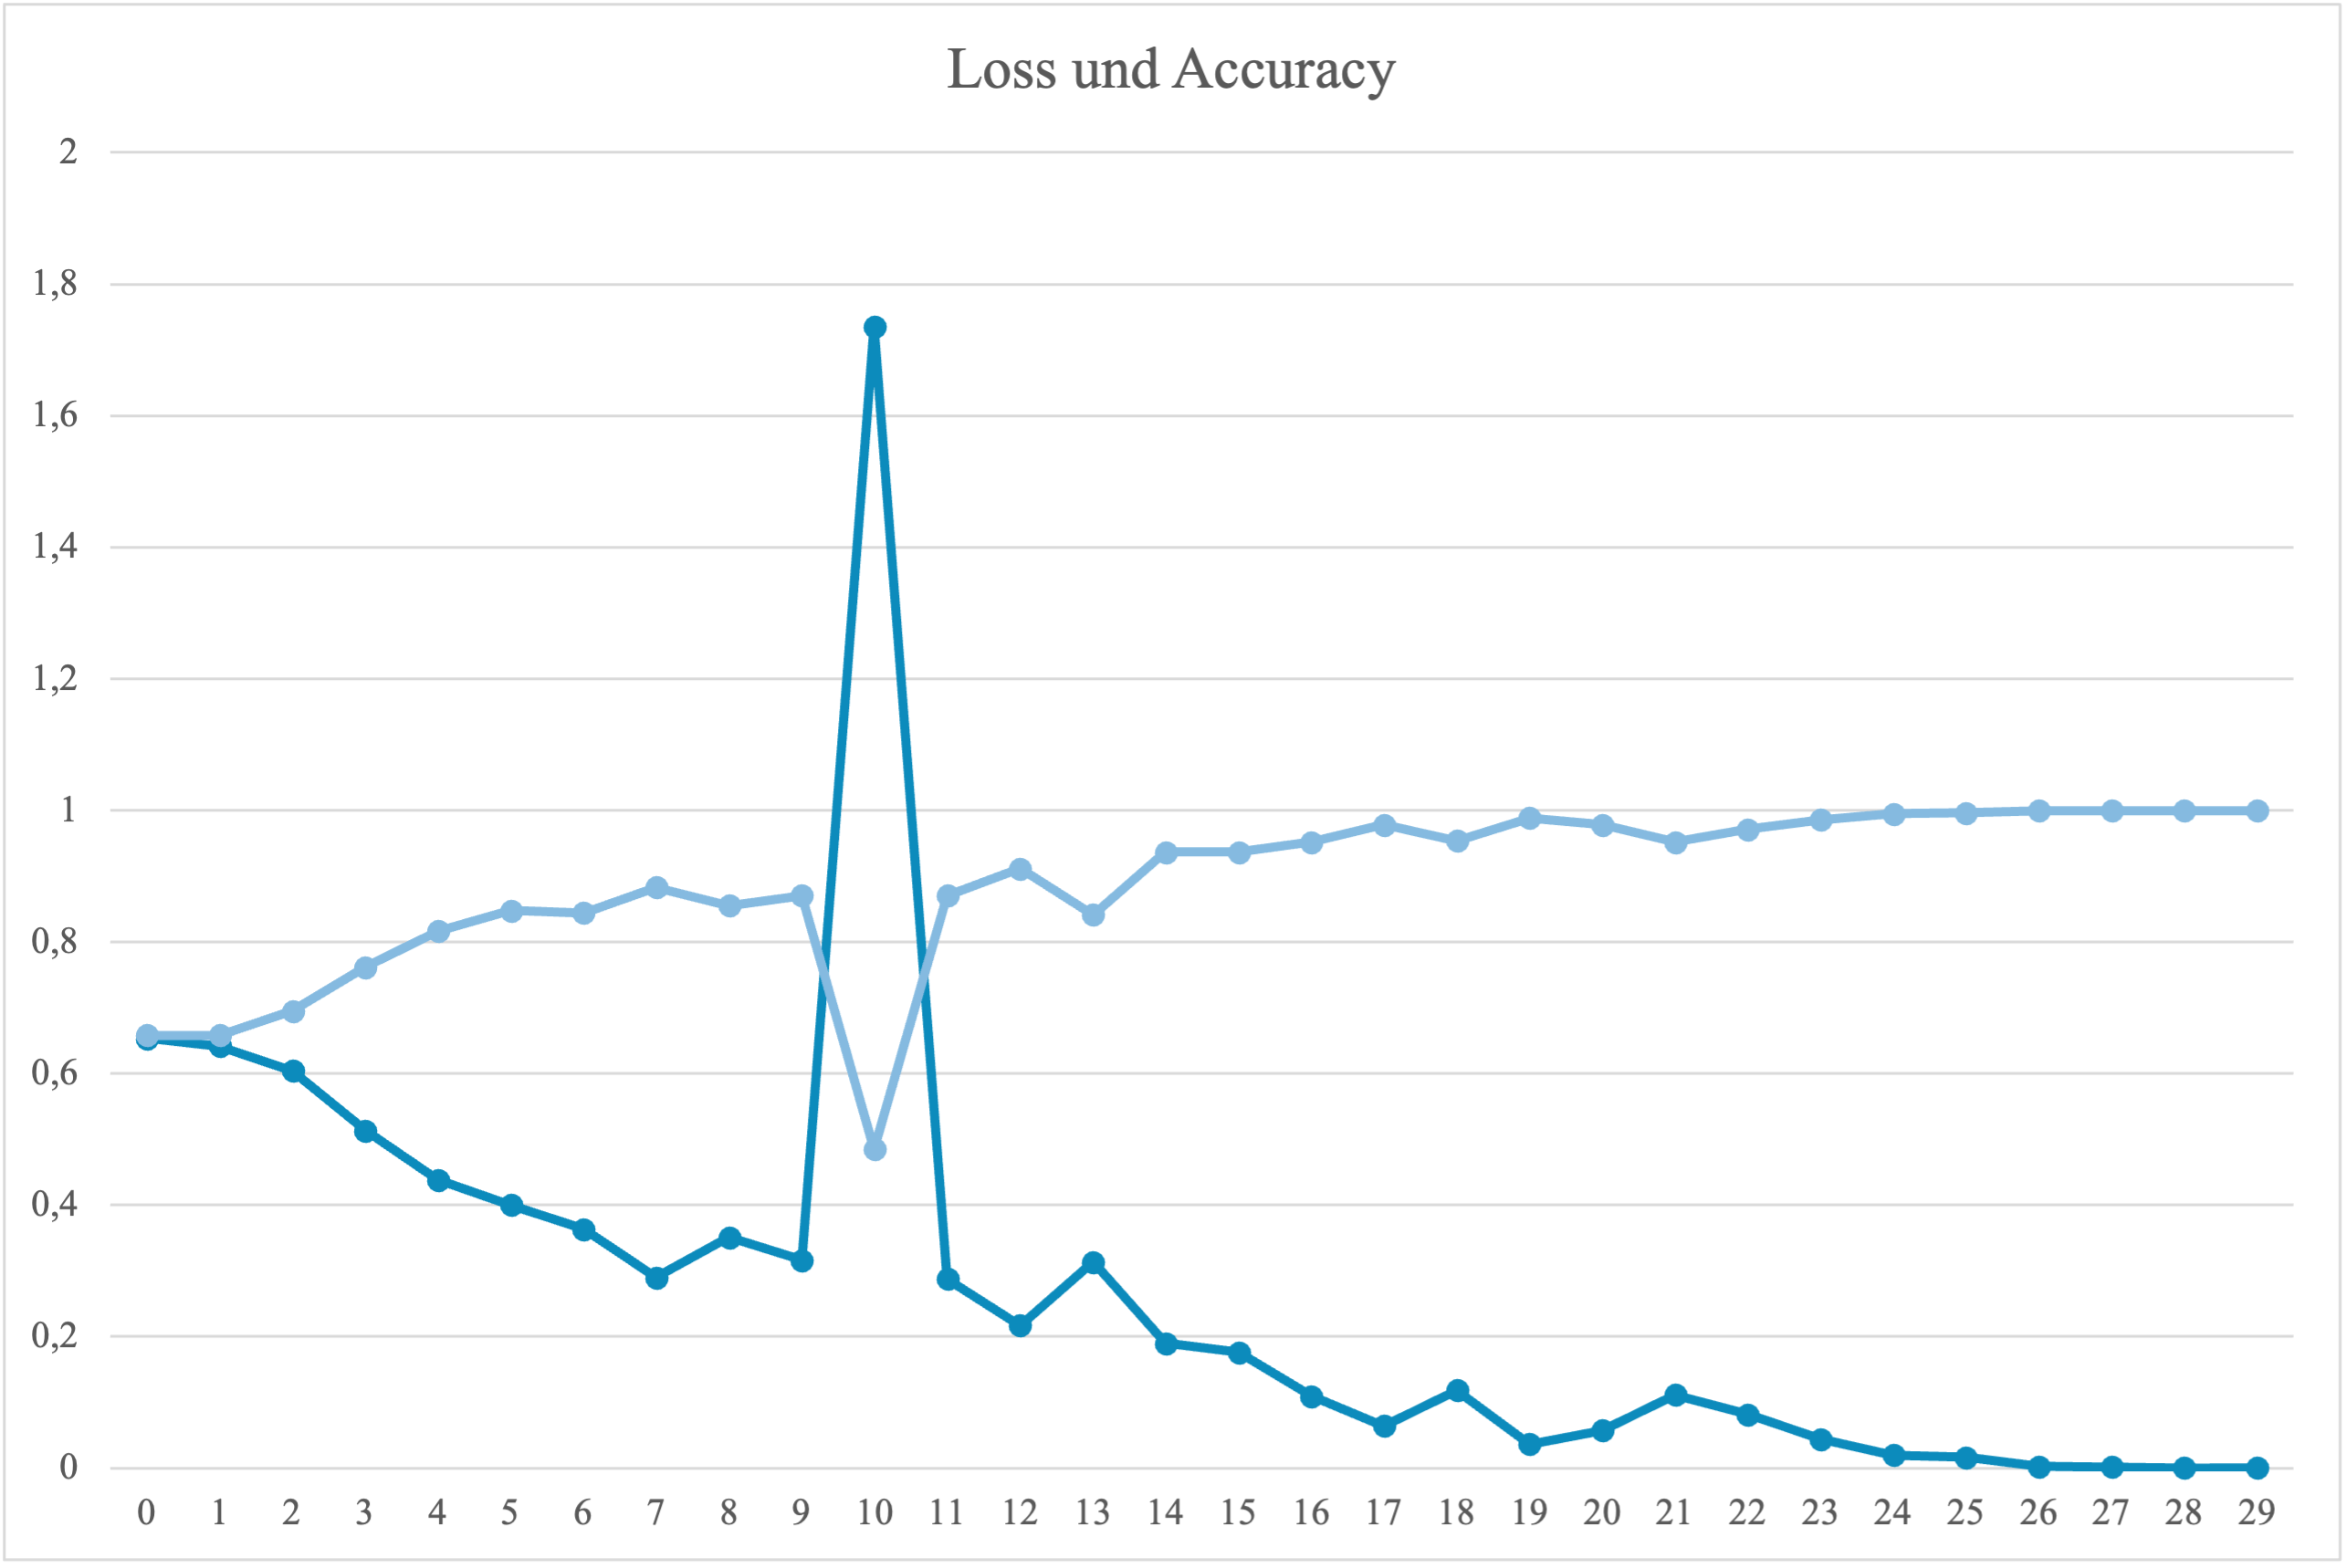
\includegraphics[width=\columnwidth]{Andi/Loss_Acc_Gewinner.png}}
    \caption{Trainingslog des CNN Modells, welches im Test die besten Ergebnisse erzielt hat.}
    \label{fig:winner}
\end{figure}

\subsection{Training und Evaluation}
Das Training des CNN-Modells wird erläutert, ebenso wie die Evaluierung der Modellleistung anhand von Metriken wie der Genauigkeit und dem Verlust.

\subsubsection{Overfitting} \label{sec:overfitting}

\section{Fazit}
Im Fazit werden die Ergebnisse der Arbeit zusammengefasst und diskutiert. Es wird reflektiert, inwiefern die gesetzten Ziele erreicht wurden und welche Verbesserungspotenziale noch bestehen.








\appendices

\section*{Appendix und die Nutzung von ergänzenden Dateien}

\section*{Danksagung}

\end{document}
